\chapter{Implementation}

\chapterintro{
  This chapter details a proof-of-concept implementation of Cloud-SAP architecture.
}

\section{Introduction}
Previous chapters detailed requirements that a self-manageable platform oriented toward Quality-of-Service assurance should comply with. Beside this, reference architecture known as Cloud-SAP was introduced. This chapter in turn highlights key elements of a proof-of-concept implementation of Cloud-SAP. Noticeably, our implementation is by all means not exhaustive and merely intends to prove that presented architecture successfully tackles raised challenges. Hence, we implemented only following subset of managers specified by Cloud-SAP:
\begin{itemize}
  \item Autonomic container manager
  \item Autonomic stack manager
  \item Autonomic cloud instance manager
  \item Autonomic cloud federation manager
\end{itemize}

Apart from that, we implemented minimal viable modules that is monitoring, analysis, planning and execution. For example, we based analysis solely on threshold model, discarding more advanced techniques that uses prediction mechanisms.

\section{Overview}
As previous section indicates, key elements of discussed implementation are as follows: autonomic container manager, autonomic stack manager, autonomic cloud instance manager, autonomic cloud federation manager. Taking their role in service deployment into account, we grouped them into auto-scaling and cloud brokerage subsystems. High level overview of system, including its internal and external elements is depicted in figure \ref{fig:hlo-implementation}. Diagram \ref{fig:csap-layers-subsystem} illustrates thee relationship between Cloud-SAP managers and above-mentioned subsystems. 

\begin{figure}[!ht]
  \begin{center}
    \includegraphics[width=\textwidth]{chapter-implementation/hlo-implementation}
  \end{center}
  \caption{High level system overview}
  \label{fig:hlo-implementation}
\end{figure}

\begin{figure}[!ht]
  \begin{center}
    \includegraphics{chapter-implementation/csap-layers-subsystem}
  \end{center}
  \caption{System parts and their relation with autonomic managers}
  \label{fig:csap-layers-subsystem}
\end{figure}

As one can see, our implementation is composed by following parts:
\begin{asparaenum}
 \item[\textbf{Auto-scaling subsystem}] Auto-scaling subsystem supervises service's life cycle, monitoring it and enacting scaling actions when necessary. It is concentrated on all service's aspects: containers, stacks and application instances thus it is in fact a group of autonomic managers composed by container, stack and cloud instance managers.

 \item[\textbf{Cloud brokerage subsystem}] Brokerage subsystem groups components that together mediates between cloud providers. In particular, it consists of:
  \begin{itemize}
   \item Cloud broker - probes cloud providers and selects best offer according to a given policy. In Cloud-SAP model, it plays a role of orchestrating autonomic manager, that is, autonomic cloud federation manager.
   \item Cloud client - delegates service provisioning request to a cloud broker.
  \end{itemize}
 
 \item[\textbf{Cloud provider}] External system that manages a group of resource such as computing nodes, storage and networking typologies. Particularly, it is able to deploy, shutdown, migrate and monitor containers. Although Cloud-SAP is utterly cloud provider independent, our implementation is solely focused on OpenNebula that uses OpenVZ as a hypervisor. We selected OpenNebula due to its simplicity, flexibility and our expertise in managing it. Choosing hypervisor, we were compelled to select one that is based on lightweight containers due to theirs flexibility in scaling as previously advocated. OpenVZ was a natural choice due to its maturity and our familiarity within it.
 
 \item[\textbf{Application provider}] An entity that is interested in application scaling and deployment. It can be represented by a human being as well as by an external system.
\end{asparaenum}

With those information in mind, we can illustrate overall architecture, components and communication protocols on deployment diagram \ref{fig:hlo-deployment}. Successive sections portrays in detail specified elements.

\section{Technology stack overview}
This section aims to give a brief outline of technologies that were used in this implementation with an endeavour to justify our choice. The chosen solutions are grouped according to their presence in appropriate subsystems.

\begin{itemize}
  \item Cloud brokerage subsystem
    \begin{asparaenum}
    \item[\textbf{Web Services/HTTP}] Communication between a client and a cloud broker is done by the usage of \emph{web services} over \emph{http} protocol. The cloud broker for a given client exposes a \emph{RESTful} API for the deployment of a service. The web service accepts \emph{JSON}-encoded messages, which comprises the name of a service and specification of each stack comprising it. The example of such a message can be found in listing \ref{lst:service-spec-test-deployment-time}.

      The reason we chose this technology is because of its simplicity, maturity and great support from Ruby platform. The other solutions that could be used in place of this one include some message-oriented middleware standards such as AMQP or JMS, other standards that facilitate communications among systems/components such as CORBA, and other such as RMI or RPC. Some of the aforementioned technologies had been eliminated once we chose Ruby as the language the platform would be implemented in. This is because of their platform-specific nature, e.g. JMS requires the system to be written in Java.

    \item[\textbf{AMQP}] Being able to communicate in an asynchronous, more scalable and loosely coupled way between a cloud broker and different cloud instance managers representing cloud providers requires the usage of message-oriented middleware. In our case we decided to use \emph{Advanced Message Queuing Protocol}as this standard is mature and its support in Ruby is solid.

      This communication channel is used in the implementation to 
      \begin{inparaenum}[a)]
      \item get offers from cloud providers for a given service and
      \item commission the cloud provider to deploy a service.
      \end{inparaenum}

    \item[\textbf{SQLite}] For the persistence layer there was a need for a lightweight database engine that would have good support in Ruby platform. Possible choices included some nonrelational solutions, such as Redis, and more traditional, relational ones, such as SQLite. We chose the latter as the drivers for \emph{DataMapper}, an ORM library, have better support in Ruby.
    \end{asparaenum}

  \item Auto-scaling subsystem
    \begin{asparaenum}
    \item[\textbf{OpenNebula}] There was a need for a tool that would be used for efficient management of the resources of a data center. OpenNebula is an open source respond to this need -- first released in 2008, with good support from the community, seemed a good candidate for a tool. Our familiarity with it was an additional factor which influenced our final choice of OpenNebula as the tool for the job.
    \item[\textbf{Chef}] As manual virtual machines provisioning is a tedious and error-prone task, this is a perfect match for a tool that would automate the process. We chose \emph{Chef} as it is written in the language of the whole platform (i.e. Ruby), mature (initially released in 2009) and widely used tool. \footnote{According to the website of the product (\url{http://www.getchef.com/customers/}), it is used by such companies as Facebook, BlueKai or BookRenter. More can be found at the provided URL.}
    \item[\textbf{OpenVZ (drivers)}] The significance of choosing linux containers as a virtualisation technology was fully described in the preceding chapters. However, the drivers for the OpenVZ are not supported by the OpenNebula maintainers, so we had to use our own-developed tool while taking a course at the university. This tools forms an official add-on for OpenNebula 3.8.
    \end{asparaenum}
\end{itemize}


\newpage
\begin{figure}[!ht]
  \begin{center}
    \includegraphics{chapter-implementation/hlo-deployment}
  \end{center}
  \caption{System's deployment diagram}
  \label{fig:hlo-deployment}
\end{figure}
\newpage

% radek
\section{Cloud brokerage subsystem}
\subsection{Introduction}
This subsystem consists of components which are directly used by a client or acts on their behalf. These are \emph{cloud client} and \emph{cloud broker} respectively. The placement of each component with annotated communication protocols can be seen in figure \ref{fig:csap-cloud-brokerage-deployment-diagram}. To annotate the cooperating components, the diagram embeds an auto-scaling subsystem node, which is not a part of this component.

\begin{figure}[!ht]
  \begin{center}
    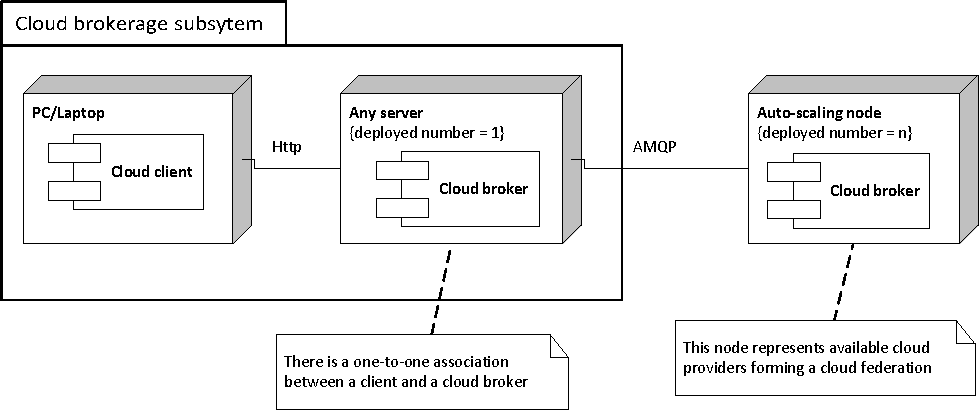
\includegraphics{chapter-implementation/csap-cloud-brokerage-deployment-diagram}
  \end{center}
  \caption{Deployment diagram of a Cloud brokerage subsystem}
  \label{fig:csap-cloud-brokerage-deployment-diagram}
\end{figure}

\subsection{Cloud client}
The client is a command line application that allows a user to communicate with a cloud broker which will further process the message and act on behalf the user. By means of this application, the user is able to deploy a service by preparing its specification in a JSON format and request its deployment to the cloud broker. Listing \ref{lst:service-spec-test-deployment-time} is an example of a service description.

The application is written purely in Ruby and uses http protocol for communication. 

\subsection{Cloud broker}
The cloud broker mediates between a client and cloud providers. Its main responsibility is to, during the deployment or scaling of a service, gather information and offers from cloud providers forming a cloud federation and choose the best, in terms of cost, providers and orders them the deployment of specific stacks comprising the service.

The broker uses Advanced Message Queuing Protocol (AMQP) for communication between itself and cloud providers. It was considered the best choice for this purpose as it ensure asynchronous message processing and sending messages according to fan-out paradigm which is ideal for this use case.

The message format is the same as in the case of a client application.

\subsubsection{Cloud providers selection}
One of the main responsibilities of the Cloud broker is to map the stacks of a given service to cloud providers. This happens when a service is to be deployed or horizontally scaled. As this implementation merely wants to be a minimal viable product, we took only the cost attribute into consideration when performing this function.

To formalize the previous statements, the problem is as follows: given a set whose elements (representing stacks) can take an non-negative values (they come from offers from cloud providers), find the mapping so as the overall sum (total cost) be minimal.

The solution is to take the minimal available price for a given stack. The simplest proof is by contradiction -- we can assume that we computed our sum using a non-minimal value for some elements. But in this case, taking the minimal value for any element causes the sum to be less than previously computed -- contradiction.

% darek
\section{Auto-scaling subsystem}

\subsection{Introduction}
The onus is on auto-scaling subsystem to:
\begin{itemize}
 \item scale applications in the most cost effective way
 \item handle application deployment requests and pass them to a cloud provider 
\end{itemize}

As overview states, this subsystem is in fact a loosely coupled group of three autonomic managers, cooperating together to achieve aforementioned subsystem's goals. System is structured (figure \ref{fig:auto-scaling-subsystem-deployment}) on top of that observation.

\begin{figure}[!ht]
  \begin{center}
    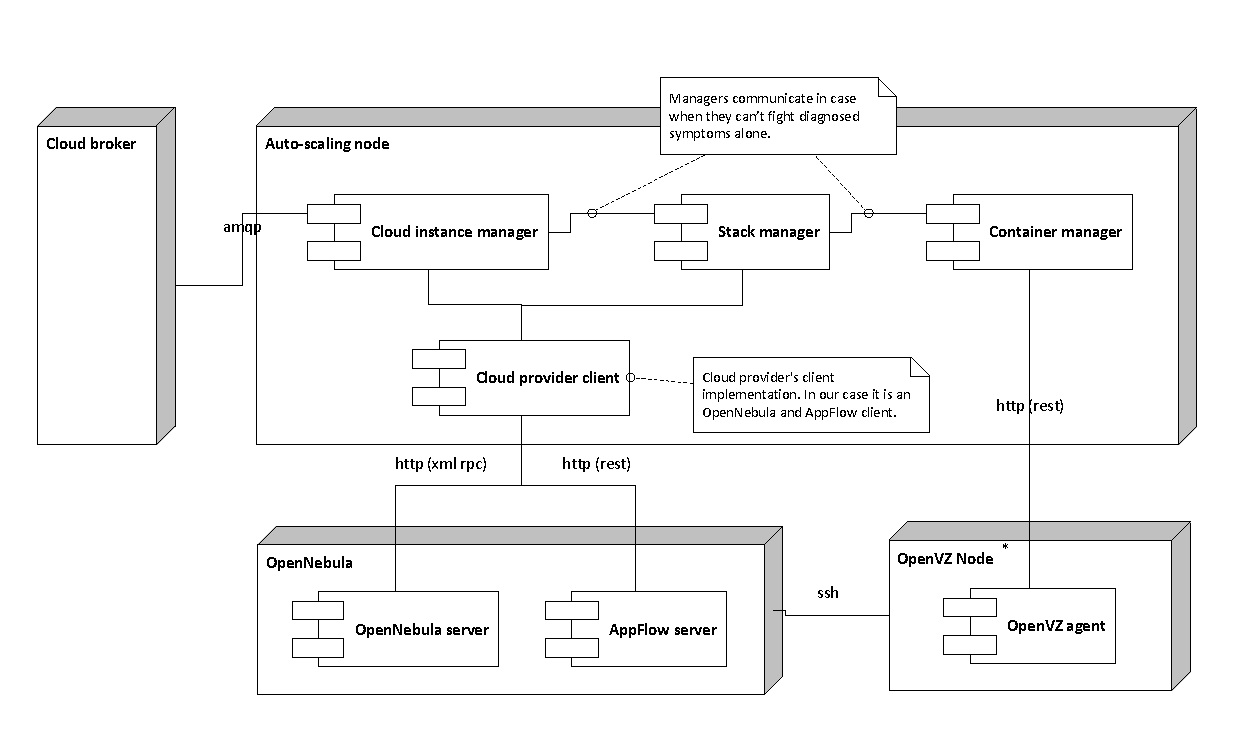
\includegraphics[width=\textwidth]{chapter-implementation/auto-scaling-subsystem-deployment}
  \end{center}
  \caption{Deployment diagram of auto-scaling subsystem}
  \label{fig:auto-scaling-subsystem-deployment}
\end{figure}

\begin{asparaenum}
 \item[\textbf{Container manager}] Manager responsible for supervising container lifecycle and taking apropriate actions when necessary. It is a most fine-grained controller in our implementation. It delegates a problem resolution to a stack manager when necessary.
 
 \item[\textbf{Stack manager}] It supervises a group of homogeneous resources, that is containers, known as a stack. Similarly to a container manager, execution may be passed to cloud instance manager when there is no choice left.
 
 \item[\textbf{Cloud instance manager}] Supervisor of a whole cloud instance correlated to a given cloud provider. It participates in dialogue with cloud broker by advertising cloud provider capabilities and handling provisioning requests. Besides, it is eligible of most coarse-grained scaling action: horizontal scaling across multiple providers.
 
 \item[\textbf{Cloud broker}] Is a part of cloud brokerage subsystem responsible for mediating between different auto-scaling subsystems and cloud client. Previous section covers it in more details.
 
 \item[\textbf{Cloud provider}] External system that provisions and manages container and underlying resources. In case of this implementation it is an OpenNebula frontend and AppFlow server, accessible through a Cloud provider client. Apart from that, OpenVZ exposes its manageability capabilities by OpenVZ agent and its REST interfaces. Next section details cloud provider.
 
 \item[\textbf{Cloud provider client}] Generic component that brings cloud provider features to a auto-scaling subsystem. Noticeably, it may be a facade to different systems, freeing subsystem from accessing cloud provider's internal structure as it is in case of our implementation. For example, it delegates service provisioning requests to an Applfow server while monitoring and scaling are passed to an OpenNebula frontend.
\end{asparaenum}

% darek
\subsection{Container manager}

\subsubsection{Objectives}
Container manager key responsibilities are as follows:
\begin{itemize}
 \item supervising container and adjusting its settings to a current usage demand, i.e. scaling it vertically
 \item delegating scaling operations to a stack manager when vertical scaling is not possible
\end{itemize}

\subsubsection{Implementation details}
Container manager is strictly related to an autonomic container manager, component specified by Cloud-SAP. Consequently, its structure reflects a control loop, cyclically invoked by a scheduler and involves:
\begin{itemize}
 \item monitoring - manager collects data from OpenNebula frontend using a cloud provider client. Currently, implementation supports following metrics:
    \begin{itemize}
     \item used cpu
     \item used memory
    \end{itemize}
    Beside this, manager aggregates collected data - it calculates its average, in case when there is more than one measurement in a cycle.
    
 \item analysis - Aggregated data is analysed against client defined policy. Policies (e.g. listing Y) are based on a threshold model, denoting a valid range for a resource measurement. Hence, its evaluation results in \texttt{FITS, LESSER, GREATER}.
 
 \item planning - During this phase, analysis conclusion is mapped to an action. Table \ref{tab:container-manager-planning} presents such mapping. As one can see, only the CPU is supported for the time being. In case of increasing CPU, resource manager is first probed to determine whether there are enough resources to perform requested action. Unless cloud provider is capable of handling request, execution is delegated to an upper layer - stack manager.
 
 \item execution - Manager adjusts container settings using an OpenVZ agent, located on computing node where container is deployed. As for OpenVZ hypervisor, container's properties are User Bean Counter (UBC), exposed through a REST interface.
\end{itemize}

\begin{table}[!htbp]
\begin{tabularx}{\textwidth}{ l  X  X }
\specialrule{.1em}{.05em}{.05em} 
\textbf{Description} & \textbf{Symptom} & \textbf{Action} \\
\specialrule{.1em}{.05em}{.05em} 

CPU exceeds upper usage limit & \texttt{GREATER\_CPU} & Increase CPU \\ \hline
CPU is in legal range & \texttt{FITS\_CPU} & None \\ \hline
CPU is lesser than allowed & \texttt{LESSER\_CPU} & Decrease CPU \\ \hline

\end{tabularx}
\caption{Container manager's analysis conclusion mappings}
\label{tab:container-manager-planning}
\end{table}

Manager constantly loops through all aforementioned phases as depicted in figure \ref{fig:contanier-lifecycle-seq}. 

\begin{figure}[!ht]
  \begin{center}
    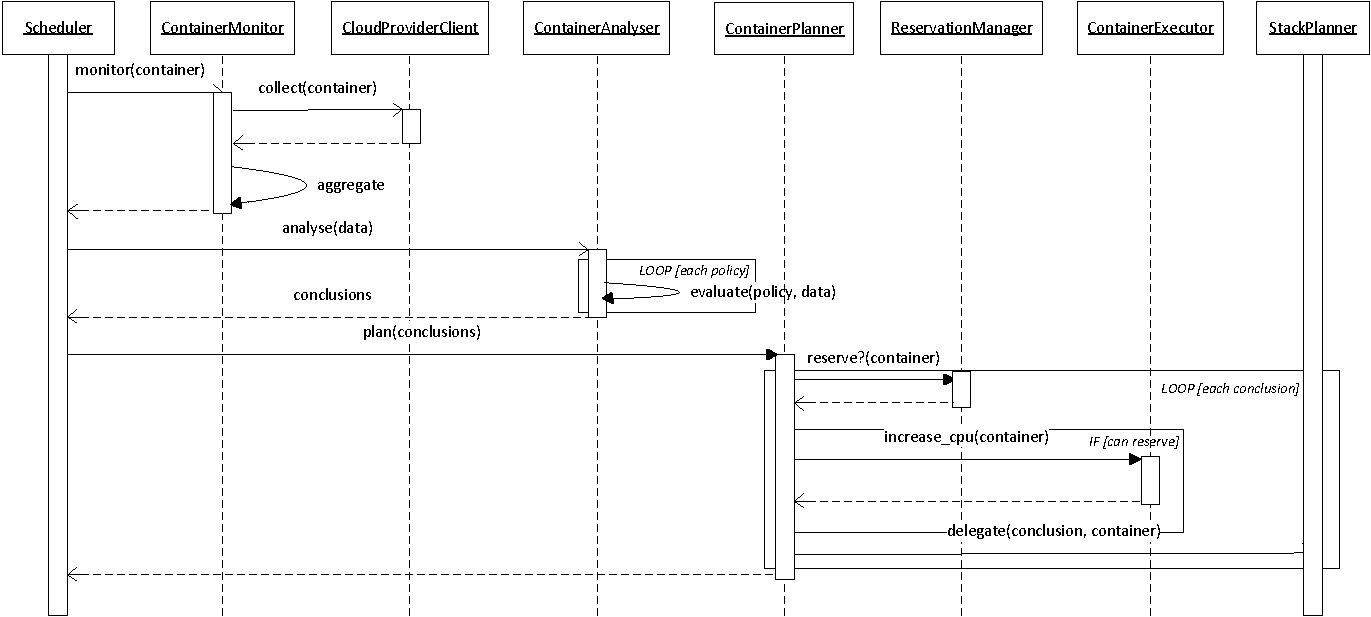
\includegraphics[width=\textwidth]{chapter-implementation/contanier-lifecycle-seq}
  \end{center}
  \caption{Sequence diagram illustrating container manager control loop}
  \label{fig:contanier-lifecycle-seq}
\end{figure}

% darek
\subsection{Stack manager}

\subsubsection{Objectives}
What lies in duties of a stack manager is:
\begin{itemize}
 \item supervising and scaling out stack
 \item delegating problem to a cloud instance manager, when not capable of resolving it
\end{itemize}

\subsubsection{Implementation details}

% radek
\subsection{Cloud instance manager}

\subsubsection{Objectives}
\begin{itemize}
  \item Processing of the deployment requests of stacks from cloud brokers
  \item Delegating the horizontal-scaling requests to the cloud broker responsible for carrying out the whole process
  \item Advertising the existence of a given cloud provider to the cloud broker
\end{itemize}

\subsubsection{Implementation details}
As all of the aforementioned objectives require a communication medium between the cloud broker and cloud instance manager, we decided to employ a message-oriented middleware solution, Advanced Message Queuing Protocol (AMQP), for this purpose. The detailed justification of this choice can be found in the section devoted to \emph{Cloud brokerage subsystem}.  

The types and formats of messages this component can process and send clearly reflects its objectives and are as follows:
\begin{asparaenum}
\item[\textbf{Deployment request message}] The message sent by a cloud broker that orders the given cloud provider to deploy a service. Data contained in the message includes the name of a service and attributes of each stack comprising it. The attributes of a stack are as follows:
  \begin{compactitem}
  \item type (e.g. java, ruby)
  \item instances (the number of virtual machines that makes the given stack)
  \item policies (scaling policies)
  \end{compactitem}
\item[\textbf{Offer request message}] The message sent by a cloud broker when it wants to retrieve the deployment capabilities of a cloud provider. It contains the attributes of the service to be deployed. They match those described in the \emph{deployment request message}.

  This manager creates an offer for a service that consists of the cost of each stack. This cost is not dynamically computed, but fetched from the configuration file that contains mapping between the stack and its cost. The offer is sent back to the cloud broker for further processing.
\item[\textbf{Horizontal-scaling message}] This message is send when it is not possible to continue having deployed a stack on the given cloud instance by the lack of sufficient resources or violation of a policy. It contains the stack specification as the platform needs this information to redeploy the stack to another cloud instance.
\end{asparaenum}

The behaviour required from the Cloud-SAP architecture regarding the control loop within the scope of \emph{monitoring} resources of a cloud provider is delegated to underlying components, stack and container managers. As this manager merely mediates between the cloud provider and broker, it does not employ any \emph{analysis} and \emph{plan} mechanisms. Conveying information forms the \emph{execute} attribute.

% darek
\subsection{Cloud provider client}


% darek
\section{Cloud provider}

% ?
\section{Exemplary scenarios}

\subsection{Service deployment}

\subsection{Scaling application}

\subsection{Scaling application across multiple cloud providers}

\section{Summary}

